%!TEX root = ../template.tex
%%%%%%%%%%%%%%%%%%%%%%%%%%%%%%%%%%%%%%%%%%%%%%%%%%%%%%%%%%%%%%%%%%%%
%% chapter3.tex
%% NOVA thesis document file
%%
%% Chapter with a short laext tutorial and examples
%%%%%%%%%%%%%%%%%%%%%%%%%%%%%%%%%%%%%%%%%%%%%%%%%%%%%%%%%%%%%%%%%%%%
\chapter{Plano de trabalhos para a Elaboração da dissertação}
\label{cha3}

%This Chapter aims at exemplifying how to do common stuff with \LaTeX. We also show some stuff which is not that common! ;)
%
% https://books.google.pt/books?id=q3DvBQAAQBAJ&pg=PA426&lpg=PA426&dq=APOD+cycle&source=bl&ots=KhoY0esEC7&sig=ecXbOBLk49T0mzgr36h1TJ9XF5I&hl=pt-PT&sa=X&ved=0ahUKEwi6g66pqIXcAhVB46QKHVcbBdkQ6AEIXzAL#v=onepage&q=APOD%20cycle&f=false
\section{Ciclo de desenvolvimento}
Tendo em conta que no decorrer da elaboração não será desenvolvido código de raiz, mas sim optimizar código existente, através de CUDA ou OpenCL, os esforços a adoptar durante a fase de elaboração seguirão um ciclo de desenvolvimento próprio para programação em GPUs, com quatro fases. Este ciclo denomina-se APOD (\textit{Assess}, \textit{Parallelize}, \textit{Optimize}, \textit{Deploy}) \cite{cudaProgGuide} e consiste em quatro fases(figura \ref{apodFig}):
\begin{enumerate}
\item {\textbf{\textit{Assess}}} : Onde é feito um \textit{assessment} ao estado atual do programa, em termos de performance. Nesta fase são determinados os pontos do programa onde este passa mais tempo a executar e identificar os bottlenecks de instruções, fazendo um profile da aplicação para confirmar as  identificações efectuadas. No caso da dissertação, é feito um profile do ficheiro bigger.lpi do open-chemera, como está descrito em \ref{profiling}. 

%Pelo que o esforço inicial para a esta etapa do ciclo já se encontra feito. Foram determinados dois pontos paralelizáveis com GPU, a detalhar em \ref{challenges}.

\item{\textbf{\textit{ Parallelize}}} : Após o \textit{assessment}  referido anteriormente estar concluido, procede-se para a fase de implementação do código para paralelizar os pontos encontrados na fase anterior. De acordo com \cite{saxpy}, existem três possibilidades para implementar acelerações: usar bibliotecas aceleradas, diretivas OpenACC ou recorrer a linguagens para programação em GPUs, como CUDA ou OpenCL. Na elaboração da dissertação é pretendido abordar a primeira e terceira possibilidades, no caso da terceira, existe a possibilidade de usar OpenCL pois é suportado pelo IDE Lazarus.

\item{\textbf{\textit{Optimize}}} : Nesta terceira fase é pretendido aumentar a performance da solução base, inicialmente esta ultima tem de ser determinada executando o programa com um dataset de tamanho adequado. E recorrer às técnicas descritas em \ref{optmi} para maximizar a performance. Também se podem considerar abstrações de outros programas relatados em \ref{gpus1}.

\item{\textbf{\textit{Deploy}}} : A última fase do ciclo consiste em confrontar a performance obtida com as expectativas fundamentadas no início do ciclo. Em caso de não corresponder ao speedup potencial registado na fase inicial, é necessário voltar à fase Assess, recomeçando o ciclo.
\end{enumerate}


     \begin{figure}[ht]
  \centering
    {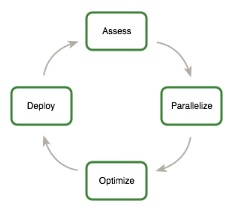
\includegraphics[width=0.5\linewidth]{APOD}}
  \caption{ Diagrama do ciclo de desenvolvimento APOD\cite{cudaProgGuide}.}
  \label{apodFig}
\end{figure}

Este ciclo de desenvolvimento será iterado o número de vezes necessário até a performance do BiGGER se enquadrar com os objetivos indicados no capitulo \ref{cap1}.
\subsection {Profiling}
\label{profiling}
Antes de se considerar opções sobre as possibilidades para efectuar a optimização do BiGGER, foi necessário fazer uma averiguação sobre o custo de cada etapa do mesmo em termos de número de chamadas e tempo total de computação. O objetivo é poder determinar zonas de codigo a paralelizar, sendo esta tarefa o acto de fazer profiling a um programa. O profiling será feito aos ficheiros relacionados com o funcionamento do BiGGER, pois existem elementos do open-chemera que não são importantes para o mesmo, como por exemplo o chemera.lpi é o que é necessário compilar e executar no Lazarus para a parte gráfica do open-chemera, não influenciando a parte do BIGGER, que é independente.  No caso do Lazarus é possivel recorrer a duas formas principais para fazer profiling a um programa:
\begin{itemize}
\item gprof : Pode-se utilizar o gprof para fazer profiling em Lazarus, gerando um ficheiro de texto com os dados necessários para averiguar quais as funções do ficheiro bigger.lpi que podem representar oportunidades de paraleliação 
\item LazProf: IDE de profiling para o lazarus, que funciona complementada com o FPProfiler 
\end{itemize}  

 A abordagem LazProfiler requer uma instalação complexa mas é a alternativa cujo profiling mostra os resultados com qualidade superior, sendo necessário apenas ordenar na interface do programa a execução do programa. A alternativa é usar o gprof, que é suportado pelo compilador FreePascal pelo que não requer uma instalação com o nivel de complexidade da do LazProfiler, no entanto os resultados não assumem a mesma qualidade do LazProfiler.
\subsection{Possibilidades de optimização} % (fold)
\label{abordagem}
O programa que serve de interface gráfica ao BiGGER, que se pode fazer a clonagem do repositório em \textit{https://github.com/lkrippahl/Open-Chemera} encontra-se implementado em Free Pascal, 97.6\% do código total, ao acordo com o que foi abordado previamente, o trabalho a realizar na elaboração incide sobre o package \textbf{\textit{docking}} mais precisamente às unidades \textbf{bogie.pas} e \textbf{dockdomains.pas}. O bogie.pas consiste no módulo de docagem geométrica  e na unidade dockdomains são determinados os dominios nos três eixos para a simulação da docagem geométrica.

 O trabalho poderá abarcar a paralelização de mais unidades presentes no pacote o que só garante melhorias adicionais à performance do Open Chemera, por exemplo na secção \ref{challenges} é abordada uma paralelização à unidade linegrids.pas, que é a unidade onde é feito o cálculo das regiões de superficie e core dos pares assim como a determinação das grelhas para a superficie 3D dos mesmos, para o efeito de complementar a resolução do desafio distipulado na secção. As principais alterações serã, no entanto, focadas nos dois referidos anteriormente.
 
Face à possibilidade de não existir nenhuma versão do CUDA para programar paralelizações em Free Pascal. %Podemos, no entanto

 Põe-se de lado esta última alternativa em troca de uma outra que recorra à framework OpenCL, que é suportada pelo Lazarus (IDE a utilizar durante a fase de elaboração do tema).
 
Poderão vir a ser implementados para a paralelização das duas unidades, kernels que executam operações de mapeamento, em que o espaço de possibilidades a tratar na primeira fase do BiGGER poderá ser associado a uma estrutura de dados(figura \ref{fig:fig3subfig}), dividida por blocos em que estes últimos serão constituidos por casas indexadas pelo ID da thread correspondente. Pelo que a indexação geral estará associada a uma fórmula que envolva a posição da thread no bloco e o número de bloco. Para cada uma das posições o core do GPU executará a função que determina se a configuração é aceite ou não.
Este esquema de indexação de threads também existe em OpenCL, por invocações próprias na sua sintaxe.
     \begin{figure}[ht]
  \centering
    {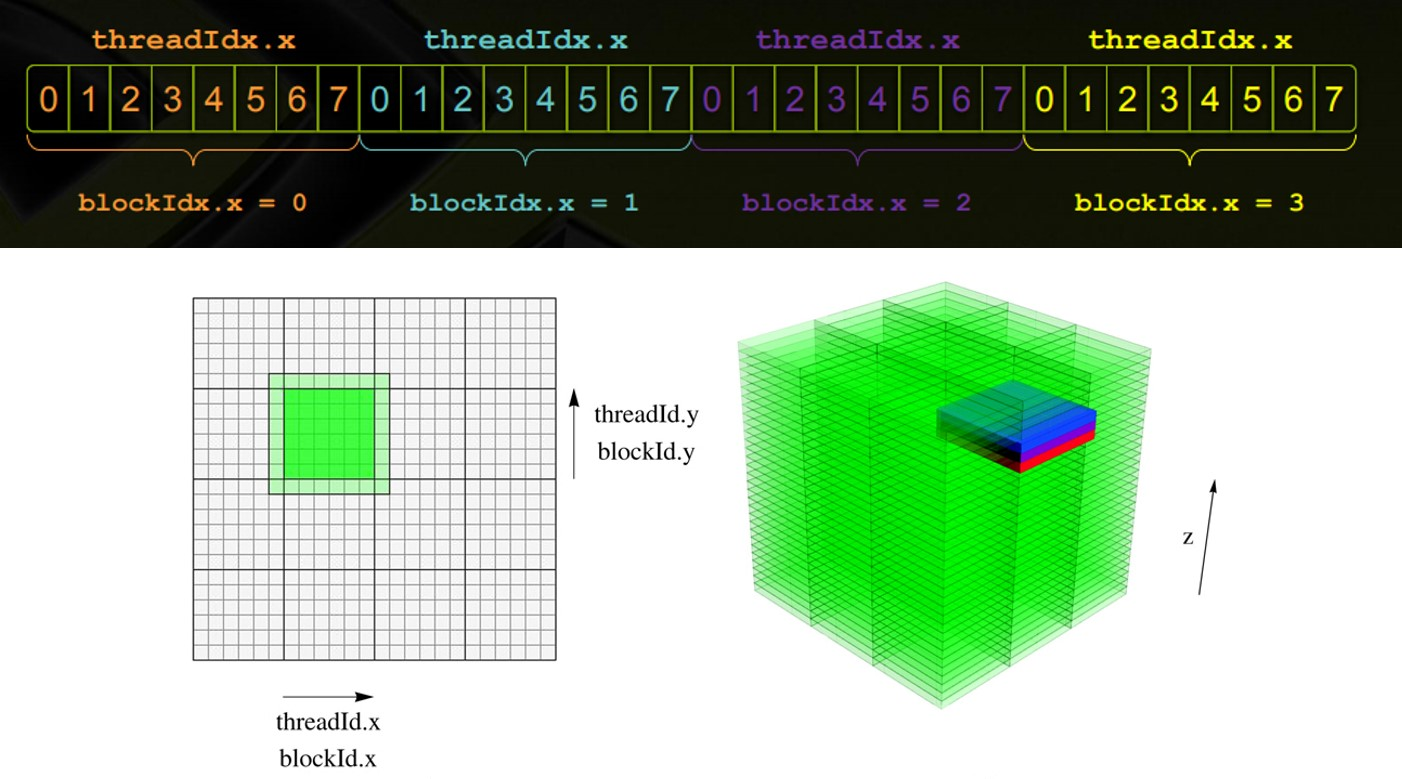
\includegraphics[width=0.5\linewidth]{Imagem1}}
  \caption{Representação gráfica do ID geral de uma thread num array divido por blocos, em CUDA. Adaptações de \cite{Sainio2010CUDAEASYA} \cite{zeller2011cuda}}
  \label{fig:fig3subfig}
\end{figure}
%continuar

\section {Desafios}
\label{challenges}
Os desafios incidem-se sobre dois pontos:
\begin{itemize}
\item{\textbf{Criação das grelhas tri-dimensionais}} : 
Tal como foi elaborado no capitulo anterior, o passo inicial do BiGGER consiste na criação de grelhas tri-dimensionais, de booleanos, que assumem valor 1 ou 0 se a posição respetiva na grelha corresponde a uma posição atómica da proteina. 

Analisando o código que se pode encontrar na unidade dockdomains.pas pode-se verificar que existem uma certa diversidade nas possibilidades de optimização.  

O código presente nesta unidade contém um conjunto de \textit{procedures} que executam cadeias de ciclos for/while, em teoria é possivel paralelizar o dockdomains recorrendo a kernels que executam operações de map, de forma a reduzir a carga de computação.

Paralelizações adicionais poderão ser feitas na unit linegrids.pas que permitem trazer melhorias extra de performance, no entanto serão alterações complementares, segundo a documentação inicial do código fonte da unidade, os segmentos gerados por esta unidade são referenciados apenas ao eixo z, sendo então uma unidade auxiliar para o BiGGER para a indexação da matriz tri-dimensional por parte deste.

\item{\textbf{Pesquisa de sobreposições}} : 
\end{itemize}
\textit{Pending Executar o profiling e apresentar resultados (1 Página com uma tabela)}
% section document_structure (end)
\section{Plano de Trabalhos} % (fold)
\label{sec:dealing_with_bibliogrpahy}
\textit{Gantt chart?}
% section dealing_with_bibliogrpahy (end)


%\section{Inserting Tables} % (fold)
%\label{sec:inserting_tables}
%
%% section inserting_tables (end)
%
%
%\section{Importing Images} % (fold)
%\label{sec:importing_images}

% section importing_images (end)


%\section{Floats, Figures and Captions} % (fold)
%\label{sec:floats_figures_and_captions}

% \subsection{Inserting Figures Wrapped with text} % (fold)
% \label{ssec:inserting_images_wrapped_with_text}
% 
% You should only use this feature is \emph{really} necessary. This means, you have a very small image, that will look lonely just with text above and below.
% 
% In this case, you must use the \verb!wrapfiure! package.  To use \verb!wrapfig!, you must first add this to the preamble:
% 
% \begin{wrapfigure}{l}{2.5cm}
%   \centering
%     
\includegraphics[width=2cm]{snowman-vectorial}
%   \caption{A snow-man}
% \end{wrapfigure}	
% 
% \noindent\verb!\usepackage{wrapfig}!\\
% This then gives you access to:\\
% \verb!\begin{wrapfigure}[lineheight]{alignment}{width}!\\
% Alignment can normally be either ``l'' for left, or ``r'' for right. Lowercase ``l'' or ``r'' forces the figure to start precisely where specified (and may cause it to run over page breaks), while capital ``L'' or ``R'' allows the figure to float. If you defined your document as twosided, the alignment can also be ``i'' for inside or ``o'' for outside, as well as ``I'' or ``O''. The width is obviously the width of the figure. The example above was introduced with:
% \lstset{language=TeX, morekeywords={\begin,\includegraphics,\caption}, caption=Wrapfig Example, label=lst:latex_example}
% \begin{lstlisting}
% 	\begin{wrapfigure}{l}{2.5cm}
% 	  \centering
% 	    
\includegraphics[width=2cm]{snowman-vectorial}
% 	  \caption{A snow-man}
% 	\end{wrapfigure}	
% \end{lstlisting}

% subsection inserting_images_wrapped_with_text (end)

% section floats_figures_and_captions (end)

%\lipsum[1-3]
%
%\begin{figure}[htbp]
%  \centering
%  \subcaptionbox{One sub-figure\label{fig:leftsubfig}}%
%    {
\includegraphics[width=0.5\linewidth]{knitting-vectorial}}%
%  \subcaptionbox{Another sub-figure\label{fig:rightsubfig}}%
%    {
\includegraphics[width=0.5\linewidth]{knitting-vectorial}}%
%  \caption{A figure with two sub-figures!}
%  \label{fig:fig2subfig}
%\end{figure}
%
%\textbf{And this is a small text that references the Figure~\ref{fig:fig2subfig} and its Subfigures~\ref{fig:leftsubfig} and~\ref{fig:rightsubfig}.}
%
%\lipsum[1-3]


%\section{Text Formatting} % (fold)
%\label{sec:text_formatting}

% section text_formatting (end)


%\section{Generating PDFs from \LaTeX} % (fold)
%\label{sec:generating_pdfs_from_latex}
%
%\subsection{Generating PDFs with pdflatex} % (fold)
%\label{ssec:generating_pdfs_with_pdflatex}
%
%You may create PDF files either by using \verb!latex! to generate a DVI file, and then use one of the many DVI-2-PDF converters, such as \verb!dvipdfm!.
%
%Alternatively, you may use \verb!pdflatex!, which will immediately generate a PDF with no intermediate DVI or PS files. In some systems, such as Apple, PDF is already the default format for \LaTeX. I strongly recommend you to use this approach, unless you have a very good argument to go for \verb!latex! + \verb!dvipdfm!.
%
%A typical pass for a document with figures, cross-references and a bibliography would be:
%\begin{verbatim}
%$ pdflatex template
%$ bibtex template
%$ pdflatex template
%$ pdflatex template
%\end{verbatim}
%You will notice that there is a new PDF file in the working directory called \verb!template.pdf!. Simple :)
%
%Please note that, to be sure all table of contents, cross-references and bibliographic citations are up-to-date, you must run \verb!latex! once, then \verb!bibtex!, and then \verb!latex! twice.
%% section generating_pdfs_with_pdflatex (end)
%
%\subsection{Dealing with Images} % (fold)
%\label{sub:dealing_with_images}
%
%You may process the same source files with both \verb!latex! or \verb!pdflatex!. But, if your text include images, you must be careful. \verb!latex! and \verb!pdflatex! accept images in different (exclusive) formats.  For \verb!latex! you may use EPS ou PS figures. For \verb!pdflatex! you may use JPG, PNG or PDF figures.  I strongly recommend you to use PDF figures in vectorial format (do not use bitmap images unless you have no other choice).
%% subsection dealing_with_images (end)


%\subsection{Creating Source Files Compatible with both latex and pdflatex} % (fold)
%\label{ssec:creating_source_files_compatible_with_both_latex_and_pdflatex}
%
%Do not include the extension of the file in the \verb!\includegraphics! command. E.g., use\\
%\verb!\includegraphics{sonwman}!\\
%and not\\
%\verb!\includegraphics{sonwman.eps}!.\\
%If you use the first form, \verb!latex! or \verb!pdflatex! will add an appropriate file extension.
%
%This means that, if you plan to use only \verb!pdflatex!, you need only to keep (preferably) a PDF version of all the images. If you plan to use also \verb!latex!, then you also need an EPS version of each image.
%% subsection creating_source_files_compatible_with_both_latex_and_pdflatex (end)
%
%% section generating_pdfs_from_latex (end)


%\newpage
%
%{\Large To be included in the sections above}\\
%
%Para fazer citações, deverá usar-se a chave da referência no ficheiro BibTeX. Se for uma única referência~\cite{Artho04}, usar um ``\verb!~!'' para ligar o \verb!\cite{...}! à palavra que o precede (\ldots\verb!referência~\cite{Artho04}!).  Caso queira fazer múltiplas citações~\cite{Shavit95,Silberschatz06,Moss85}, deverá agrupá-las dentro de um úinico \verb!\cite{...}!.
%
%Note que o ficheiro de bibliografia pode ter tantas entradas quantas quiser. Apenas aquelas cuja chave seja referenciada no texto é que serão incluidas na listagem de bibliografia.
%
%
%Footnotes\footnote{This is a simple footnote.} will be numbered and shown in the bottom of the page.
%
%
%A Tabela~\ref{tab:hla:results} ilustra alguns conceitos importantes associados à contrução de tabelas:
%\begin{asparaenum}[i)]
%	\item Não usar linhas verticais;
%	\item A legenda deve ficar por cima da tabela;
%	\item Usar as macros \verb!\toprule!, \verb!\midrule! e \verb!\bottomrule! para fazer a linha horizontal superior, interiores e inferior, respectivamente.
%\end{asparaenum}
% 
%\begin{table}[ht]
%	\caption{Test results summary.}
%	\label{tab:hla:results}
%\centering
%\begin{tabular}{lccccc}
%	\toprule
%	\multicolumn{1}{c}{\textbf{Test}} 	& \textbf{Anomalies}	& \textbf{Warnings}	& \textbf{Correct} 	& \textbf{Categories}		& \textbf{Missed} \\
%	\midrule
%\cite{Beckman08}~Connection 	& 2 & 2	& 1	& \emph{C}				& 1 \\
%\cite{Artho03}~Coordinates'03 	& 1	& 4	& 1	& \emph{2B, 1C}			& 0 \\
%\cite{Artho03}~Local Variable	& 1	& 2	& 1	& \emph{A}				& 0 \\
%\cite{Artho03}~NASA				& 1	& 1	& 1	& ---					& 0 \\
%\cite{Artho04}~Coordinates'04	& 1	& 4	& 1	& \emph{3C}				& 0 \\
%\cite{Artho04}~Buffer			& 0	& 7	& 0	& \emph{2A, 1B, 2C, 2D}	& 0 \\
%\cite{Artho04}~Double-Check		& 0	& 2	& 0	& \emph{1A, 1B}			& 0 \\
%\cite{Flanagan04}~StringBuffer	& 1	& 0	& 0	& ---					& 1 \\
%\cite{Praun03}~Account			& 1	& 1	& 1	& ---					& 0 \\
%\cite{Praun03}~Jigsaw			& 1	& 2	& 1	& \emph{C}				& 0 \\
%\cite{Praun03}~Over-reporting	& 0	& 2	& 0	& \emph{1A, 1C}			& 0 \\
%\cite{Praun03}~Under-reporting	& 1	& 1	& 1	& ---					& 0 \\
%\cite{IBM-Rep}~Allocate Vector	& 1	& 2	& 1	& \emph{C}				& 0 \\
%Knight Moves					& 1	& 3	& 1	& \emph{2B}				& 0 \\
%	\midrule
%	\textbf{Total}			& \textbf{12}		& \textbf{33}		& \textbf{10}			& \textbf{5A, 6B, 10C, 2D}	& \textbf{2} \\
%	\bottomrule
%\end{tabular}
%\end{table}
%
%
%As figuras a inserir no documento deverão ser de qualidade, preferencialmente em formato vectorial (PDF vectorial) e não em \emph{bitmap} (PNG, JPG, etc). As imagens \emph{bitmap} (Figura~\ref{fig:Figuras_Tree_silhouettes-bitmap}) não escalam bem e têm reflexos negativos na qualidade do seu docuemnto.  Pelo contrário, as imagens \emph{vectoriais} {Figura~\ref{fig:Figuras_Tree_silhouettes-vectorial}} escalam muito tanto quanto o necessário sem degradar a qualidade da imagem.
%
%Só deve usar \emph{screenshots} se não tive mesmo nenhuma alternativa.  Em vez e gerar um \emph{screenshot}, tente usar uma impressora virtual PDF e imprimir para um ficheiro PDF. Regra geral obterá um PDF vetorial. Mesmo que o seu PDF contenha imagens, elas terão sempre qualidade maior ou igual à que obteria com um \emph{screenshot}.
%
%
%\begin{figure}[htbp]
%	\centering
%	
\includegraphics[height=1in]{snowman-bitmap}
%	
\includegraphics[height=3in]{snowman-bitmap}
%	
\includegraphics[height=6in]{snowman-bitmap}
%	\caption{Imagem em formato \emph{bitmap} (JPG)}
%	\label{fig:Figuras_Tree_silhouettes-bitmap}
%\end{figure}
%
%\begin{figure}[htbp]
%	\centering
%	
\includegraphics[height=1in]{snowman-vectorial}
%	
\includegraphics[height=3in]{snowman-vectorial}
%	
\includegraphics[height=6in]{snowman-vectorial}
%	\caption{Imagem em formato PDF vectorial}
%	\label{fig:Figuras_Tree_silhouettes-vectorial}
%\end{figure}
%
%Para agregar várias figuras numa única… Poderá assim referenciar o conjunto~\ref{fig:figura-completa}, a priemira delas~\ref{fig:novelo} ou a segunda~\ref{fig:nuvem}.
%
%
%\begin{figure}[htbp]
%	\centering
%    \subbottom[Novelo de lã] {%
%		\label{fig:novelo}
%		
\includegraphics[height=1in]{knitting-vectorial}
%    }
%\qquad\qquad
%    \subbottom[Tempestade com neve] {%
%		\label{fig:nuvem}
%		
\includegraphics[height=1in]{snowstorm-vectorial}
%    }
%  \caption{Exemplo de utilização de \emph{subbottom}}
%  \label{fig:figura-completa}
%\end{figure}
%
%
%Para incluir listagens de código no seu documento, deverá incluir o pacote \emph{listings} e depois usar o ambiente \emph{lstlisting}, como exemplificado na Listagem~\ref{lst:HelloWorld}.
%
%\lstset{language=Java, caption=Hello World, label=lst:HelloWorld}
%\begin{lstlisting}
%/** 
% * The HelloWorldApp class implements an application that
% * simply prints "Hello World!" to standard output.
% */
%class HelloWorldApp {%
%    public static void main(String[] args) {%
%        System.out.println("Hello World!"); // Display the string.
%    }
%}
%\end{lstlisting}
%
%\section{Equações}
%
%O LaTeX é uma ferramenta poderosa para escrever em estilo matemático. Permite inserir fórmulas no meio do texto como por exemplo esta: $ax^2 + bx + c = 0$. Também permite que as fórmulas sejam destacadas numa linha separada e centradas na página 
%$$x = \frac{-b \pm \sqrt{b^2-4ac}}{2a}$$
%\[x = \frac{-b \pm \sqrt{b^2-4ac}}{2a}\]
%ou numeradas 
%\begin{equation}
%aaa
%\label{eq:1}
%\end{equation}
%que depois pode ser referida no texto como sendo a equação~\ref{eq:1}
%$$\begin{array}{l}
%aa
%\end{array}
%$$
%
%\begin{eqnarray}
%a\\
%b\\
%c\\
%\end{eqnarray}
